\documentclass{standalone}
\usepackage{hsbcommon}
\begin{document}
    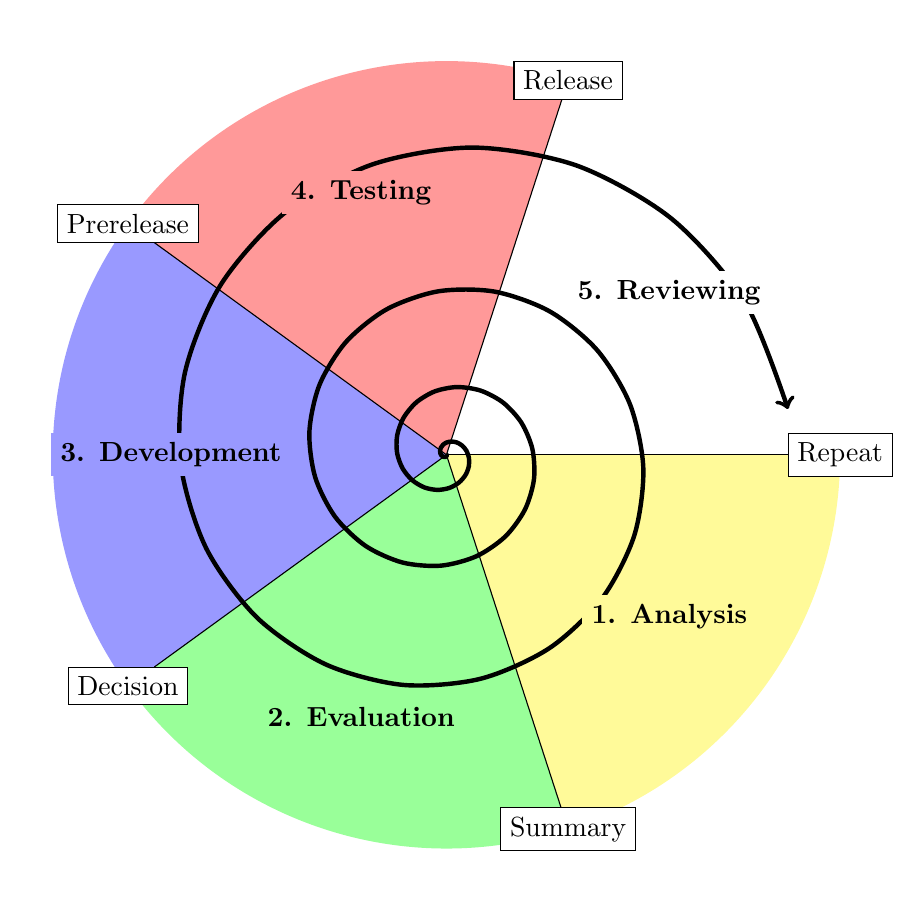
\begin{tikzpicture}
        \def\phi{72};
        \foreach [count=\i] \farb in {yellow, green, blue, red, white}
            \filldraw[fill=\farb!40,draw=none] (0:0) -- (-\i*\phi:5) arc (-\i*\phi:-\i*\phi+\phi:5) -- cycle;
            \draw[->,ultra thick] [domain=0:25,variable=\t,smooth,samples=75]
        plot ({-\t r}: {0.007*\t*\t});
        \foreach [count=\i] \farb/\m/\n in {yellow/Analysis/Summary, green/Evaluation/Decision, blue/Development/Prerelease, red/Testing/Release, white/Reviewing/Repeat}
        {
            \node[fill=\farb!40] at (-\i*\phi+\phi/2:3.5) {\textbf{\i. \m}};           
            \node[fill=white,draw] (mile\n) at (-\i*\phi:5) {\n};           
            \draw (mile\n) -- (0:0);
        }

    \end{tikzpicture}

\end{document}
